\chapter{EARLY INVESTIGATION: HARDWARE ABSTRACTION}
\label{hardware}
The initial research for this thesis into the domain of SDN was based on
the utilization of frameworks that provide low level access to networking
resources. In order to maintain high performance and control in user level
application space, these devices need to be abstracted. Network interfaces,
both logical and physical, can expose a variety of capabilities and features
that need to be properly encapsulated. This chapter discusses the evaluation of
low level port abstractions provided by DPDK (Section \ref{hardware:dpdk}) and
Netmap (Section \ref{hardware:netmap}) mid-level port abstractions implemented
in ODP (Section \ref{hardware:odp}) as well as the conclusions drawn in Section
\ref{hardware:concl}.

\section{DPDK}
\label{hardware:dpdk}
Intel's DPDK provides users with a framework on which data plane applications
can be built utilizing highly optimized constructs and device drivers. At the
time of this investigation, the project was in the early stages of development
(version 1.0, 1.1). The drivers provided by the development kit are written
specifically for Intel brand networking devices. Systems that lack compatible
hardware can provision a virtual machine to take advantage of the optimized
port drivers available. In order to execute an application with the DPDK runtime
environment, the host operating system requires some additional modifications
as well. A custom networking kernel module allows applications to bypass the
host systems native networking stack, reducing the number of copies made
between user and kernel space. Memory page size is also increased to reduce
the number of page faults.

\begin{figure}[h!]
  \centering
  \begin{subfigure}[b]{0.48\textwidth}
    \centering
    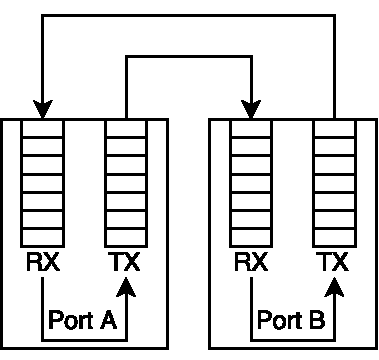
\includegraphics[scale=0.9]{dpdk_l2_a}
    \caption{Default L2 forwarding behavior.}
  \end{subfigure}
  \hfill
  \begin{subfigure}[b]{0.48\textwidth}
    \centering
    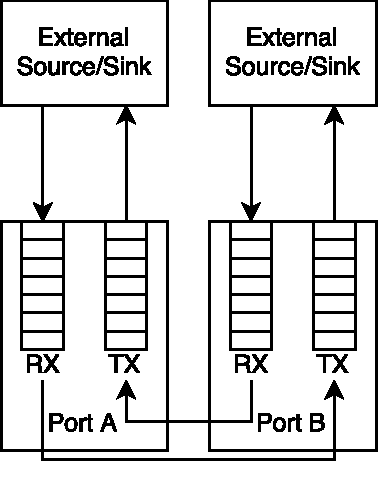
\includegraphics[scale=0.9]{dpdk_l2_b}
    \caption{Modified L2 forwarding behavior.}
  \end{subfigure}
  \caption{DPDK L2 forwarding driver.}
  \label{dpdk_l2}
\end{figure}

The goal of the experiment is to create a virtual ``wire'' between two Ethernet
ports, such that data received by port A is sent by port B, and vice versa. An
example application, L2 Forward, provided in the development kit served as a
starting point for this experiment. The example creates an \emph{external}
wire between pairs of ports, where port A sends data to port B, and B sends to
A. In order to create an \emph{internal} wire, the driver for each port needed
to be changed. Figure \ref{dpdk_l2} illustrates the behavior models used in the
experiment. The modified implementation has each port reading from it's
counterpart's receive queue and sending a copy from itself.  The destination
address fields have to be re-factored from being statically hard coded in the
port driver to a dynamic, mutable property.

Execution of the modified application gives inconsistent results, and can
require system restarts between runs to reconfigure the virtual machine when
errors occur. This is attributed to performance and abstraction penalties
suffered from the use of the virtual machine as the runtime environment host.
Though DPDK's optimized port drivers deliver solid performance,
the results show that utilizing this framework for abstracting low level port
resources would narrow the field of compatible physical devices to target.

\begin{figure}[h!]
  \centering
  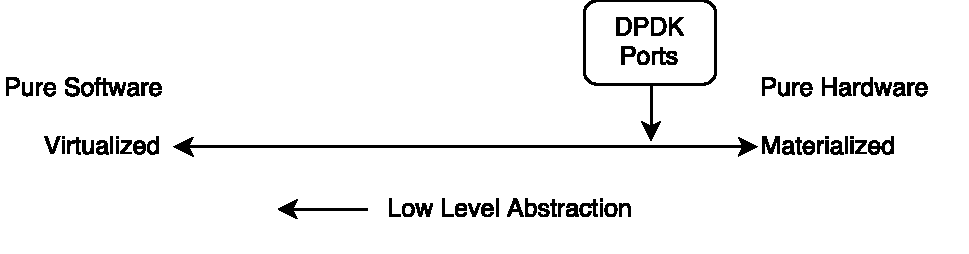
\includegraphics[scale=0.75]{spectrum_dpdk}
  \caption{DPDK's port abstraction on the spectrum.}
  \label{hardware:spectrum_dpdk}
\end{figure}

\section{Netmap}
\label{hardware:netmap}
The second framework evaluated for port abstraction comes from the Netmap
project. Netmap provides low level access to network interfaces by diverting
the flow of data to and from the interface away from the operating system, and
towards a custom device. Receive and transmit queues are mapped into user space
where the raw data can be operated on directly rather than through the operating
system network stack. Figure \ref{hardware:netmap_overview} illustrates the
mechanism provided by Netmap.

\begin{figure}[h!]
  \centering
  \begin{subfigure}[b]{0.48\textwidth}
    \centering
    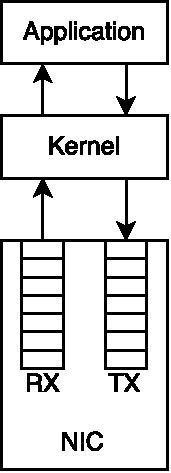
\includegraphics[scale=0.9]{netmap_overview_a}
    \caption{User space applications use the kernel to access resources.}
  \end{subfigure}
  \hfill
  \begin{subfigure}[b]{0.48\textwidth}
    \centering
    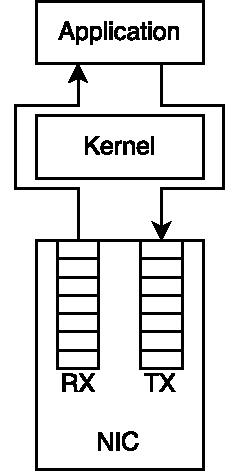
\includegraphics[scale=0.9]{netmap_overview_b}
    \caption{Netmap gives direct access to hardware memory resources.}
  \end{subfigure}
  \caption{Netmap driver functionality.}
  \label{hardware:netmap_overview}
\end{figure}

The portability factor makes Netmap a great candidate for a low level port
abstraction framework, supporting hardware NIC, logical (e.g. UDP, TCP,
UNIX sockets), and virtual (provided by the Netmap VALE software switch) ports.
Moving the memory address space for a network device into user space eliminates
the need for coherency resolution through the operating system kernel, and gives
an increase in performance while processing raw packet data. However there is a
lack of control over the networking interfaces to allow applications to monitor
the state and alter the configuration of ports. Netmap ports are currently
supported by the Freeflow port abstraction to overcome the missing
functionality.

\begin{figure}[h!]
  \centering
  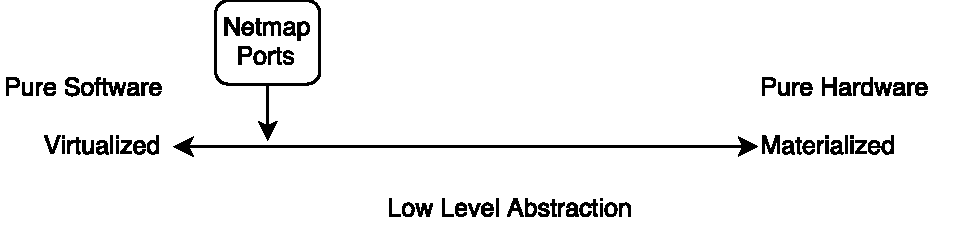
\includegraphics[scale=0.75]{spectrum_netmap}
  \caption{Netmap's port abstraction on the spectrum.}
  \label{hardware:spectrum_netmap}
\end{figure}

\section{ODP}
\label{hardware:odp}
The OpenDataPlane project provides an API for programming network data plane
applications across multiple platforms. Currently, software implementations
exist for Linux and DPDK back ends as references for design and integration
purposes. ODP allows for different back ends in order to support a broader class
of networking devices. Figure \ref{hardware:odp_overview} shows the possible
architectural models that can be constructed using ODP.

\begin{figure}[h!]
  \centering
  \begin{subfigure}[b]{0.48\textwidth}
    \centering
    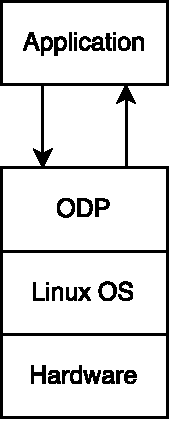
\includegraphics[scale=0.9]{odp_overview_a}
    \caption{ODP and Linux APIs expose the underlying hardware to applications.}
  \end{subfigure}
  \hfill
  \begin{subfigure}[b]{0.48\textwidth}
    \centering
    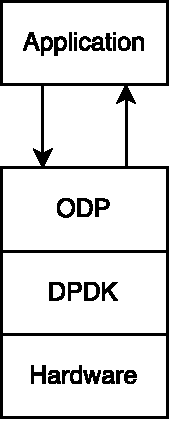
\includegraphics[scale=0.9]{odp_overview_b}
    \caption{ODP and DPDK provide accelerated driver support to applications.}
  \end{subfigure}
  \caption{ODP framework.}
  \label{hardware:odp_overview}
\end{figure}

ODP's aim to provide flexibility and performance is mirrored in the design of the
FFVM, and support for the framework is being investigated. The C API exposed gives
enough user space control over networking interfaces while minimizing the
performance cost incurred by hardware abstraction. Integration of ODP ports
into the FFVM port abstraction is currently being evaluated. Figure
\ref{hardware:spectrum_odp} shows where ODP's port implementation falls in the
virtualization-materialization spectrum.

\begin{figure}[h!]
  \centering
  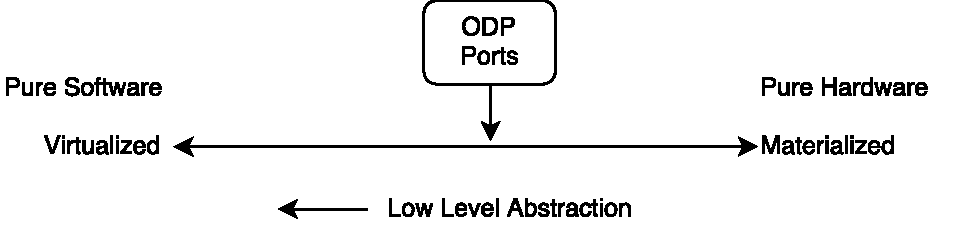
\includegraphics[scale=0.75]{spectrum_odp}
  \caption{ODP's port abstraction on the spectrum.}
  \label{hardware:spectrum_odp}
\end{figure}

\section{Conclusions}
\label{hardware:concl}
During these three investigations, the design and implementation of the FFVM
port abstraction evolved. The proper level of abstraction lies just above the
middle of the virtualization-materialization spectrum, where programmers can
maintain a high level of control over networking interfaces while utilizing
optimized operational mechanisms provided in the target system.

% Figure
% \ref{hardware:spectrum_ffports} plots the current region FFVM ports occupy.

% \begin{figure}[h!]
%   \centering
%   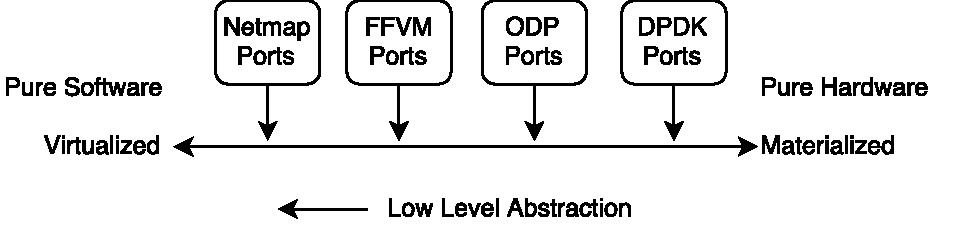
\includegraphics[scale=0.75]{spectrum_ffports}
%   \caption{The Freeflow VM port abstraction plotted along side the other
%   frameworks investigated.}
%   \label{hardware:spectrum_ffports}
% \end{figure}
